\documentclass{article}

%%%%%%%%%%%%%%%%%%%%%%%%%%%%%%%%
% PACKAGES
%%%%%%%%%%%%%%%%%%%%%%%%%%%%%%%%
\usepackage{times}
\usepackage{fullpage}
\usepackage{latexsym}
\usepackage{amsmath}
\usepackage{amssymb}
\usepackage{mathtools}
\usepackage{accents}
\usepackage{tikz}
\usepackage{pgfplots}
\usepackage[ruled]{algorithm}
\usepackage{algpseudocode}
\usepackage{dsfont}
\usepackage[bf]{caption}
\usepackage{hyperref}
\hypersetup{
    bookmarks=true,         % show bookmarks bar?
    unicode=false,          % non-Latin characters in AcrobatÕs bookmarks
    pdftoolbar=true,        % show AcrobatÕs toolbar?
    pdfmenubar=true,        % show AcrobatÕs menu?
    pdffitwindow=false,     % window fit to page when opened
    pdfstartview={FitH},    % fits the width of the page to the window
    pdftitle={My title},    % title
    pdfauthor={Author},     % author
    pdfsubject={Subject},   % subject of the document
    pdfcreator={Creator},   % creator of the document
    pdfproducer={Producer}, % producer of the document
    pdfkeywords={keyword1} {key2} {key3}, % list of keywords
    pdfnewwindow=true,      % links in new window
    colorlinks=true,       % false: boxed links; true: colored links
    linkcolor=red,          % color of internal links (change box color with linkbordercolor)
    citecolor=blue,        % color of links to bibliography
    filecolor=magenta,      % color of file links
    urlcolor=cyan           % color of external links
}
\usepackage{amsthm}
\usepackage{natbib}
\usepackage[capitalize]{cleveref}
\usepackage{graphicx}
\usepackage{parskip}
\usepackage{tikz} 
\usetikzlibrary{arrows,positioning} 
\pgfarrowsdeclarecombine{ring}{ring}{}{}{o}{o}
%\DeclareMathOperator{\ringarrow}{\raisebox{0.5ex}{\tikz[baseline]{\draw[ring->](0,0)--(2em,0);}}}
%%%%%%%%%%%%%%%%%%%%%%%%%%%%%%%%
% MACROS
%%%%%%%%%%%%%%%%%%%%%%%%%%%%%%%%
\newcommand{\defined}{\vcentcolon =}
\newcommand{\rdefined}{=\vcentcolon}
\newcommand{\E}{\mathbb E}
\newcommand{\Var}{\operatorname{Var}}
\newcommand{\calF}{\mathcal F}
\newcommand{\sr}[1]{\stackrel{#1}}
\newcommand{\set}[1]{\left\{#1\right\}}
\newcommand{\ind}[1]{\mathds{1}\!\!\set{#1}}
\newcommand{\argmax}{\operatornamewithlimits{arg\,max}}
\newcommand{\argmin}{\operatornamewithlimits{arg\,min}}
\newcommand{\floor}[1]{\left \lfloor {#1} \right\rfloor}
\newcommand{\ceil}[1]{\left \lceil {#1} \right\rceil}
\newcommand{\eqn}[1]{\begin{align}#1\end{align}}
\newcommand{\eq}[1]{\begin{align*}#1\end{align*}}
\newcommand{\Ber}{\operatorname{Bernoulli}}
\renewcommand{\P}[1]{\operatorname{P}\left\{#1\right\}}

\tikzset{
    %Define standard arrow tip
    >=stealth',
    %Define style for boxes
    observed/.style={
           circle,
           rounded corners,
           draw=black, thick,
           minimum width=1em,
           minimum height=1em,
           font=\footnotesize,
           text centered,
           fill=blue!20!white},
     latent/.style={
           circle,
           rounded corners,
           draw=black, thick, dashed,
           minimum width=.5em,
           minimum height=.5em,
           font=\footnotesize,
           text centered,
           fill=black!10!white
           },
    % Define arrow style
    pil/.style={
           o->,
           thick,
           shorten <=2pt,
           shorten >=2pt,},
    sh/.style={ shade, shading=axis, left color=red, right color=green,
    shading angle=45 }  
}


%%%%%%%%%%%%%%%%%%%%%%%%%%%%%%%%
% THEOREMS
%%%%%%%%%%%%%%%%%%%%%%%%%%%%%%%%
\theoremstyle{plain}
\newtheorem{theorem}{Theorem}
\newtheorem{proposition}[theorem]{Proposition}
\newtheorem{lemma}[theorem]{Lemma}
\newtheorem{corollary}[theorem]{Corollary}
\theoremstyle{definition}
\newtheorem{definition}[theorem]{Definition}
\newtheorem{assumption}[theorem]{Assumption}
\newtheorem{remark}[theorem]{Remark}
\newtheorem{example}[theorem]{Example}

\begin{document}
\def\ci{\perp\!\!\!\perp}

\section*{Observe then pick best}
\begin{itemize}


\item Assume we have $K$ bernoulli arms with means ordered from highest to lowest $\mu_1 ... \mu_K$. Let $\Delta = [\Delta_1...\Delta_K]$ be the differences from the optimal reward $\mu_1$. 

\item The goal is to bound the psuedo-regret upto a total number of timesteps $T$

\item Our algorithm will explore by playing uniformly at random for $h$ timesteps and then select the arm with the highest estimated reward for the remaining timesteps $T-h$.

\item We assume each arm corresponds to setting one binary input variable $X_j$ to a given value. All the input variables are assumed to be independent causes of the binary reward variable $Y$. With this structure the probability of a reward is the same under the observation that a variable takes a given configuration as under the action that assigns it. Therefore, for each exploration timestep, we get data on the performance of half of the arms. 

\item We assume $P(X_j = 1) = \frac{1}{2} \forall j$. With this assumption we will have $n_i \sim Binomial(h,\frac{1}{2})$ observations for each arm $i$ at the end of the exploration stage. Note that this is independent of the number of arms $K$. Relaxing this assumption will require us to have a more targeted exploration phase - as otherwise we do not gain any information about the value of arms that do not occur naturally with reasonable probability. 
\end{itemize}


\subsection*{Regret during explore phase}
Since the probability we play each arm is constant and uniform during the exploration phase, the expected regret is simply proportional to the average sub-optimality $\Delta$.
\eqn{
R_1 = h\sum_i P(i)\Delta_i = \frac{h}{K}\sum_i \Delta_i = h E[\Delta]
}

\subsection*{Regret during exploit phase}
The regret during this phase is proportional to the expected sub-optimality of the arm with the highest empirical mean at the end of the explore phase.

\eqn{
\hat{i^*} = argmax_i [\hat{\mu}_i]
}
\eqn{
R_2 = (T-h)E[\Delta_{\hat{i^*}}] = (T-h)\sum_i P(\hat{\mu}_i \geq \hat{\mu}_j \forall j)\Delta_i 
}

The difficulty with this approach is that it is hard to get bounds that are tight for all $\Delta$. Instead, we will bound the probability that we select an arm with a sub-optimality gap greater than some $D$.
\eqn{
R_2 \leq (T-h)\left(P(\Delta_{\hat{i^*}} \leq D) D+P(\Delta_{\hat{i^*}} > D)  \Delta_{max} \right)
}
The goal now is to get a bound for $P(\Delta_{\hat{i^*}} > D)$ in terms of Hoeffdings type bounds for each arm. 

Suppose $i = \hat{i^*} \implies \hat{\mu}_i > \hat{\mu}_1$. If we haven't over-estimated $\mu_i$ too much, $\hat{\mu}_i - \mu_{i} < \frac{D}{2}$, and haven't under-estimated $\mu_1$ too much, $\mu_1 - \hat{\mu_1} < \frac{D}{2}$, then $\Delta_{\hat{i^*}} = \mu_1 - \mu_i < D$

\eqn{
\label{eqn:probDeltaToLarge}
P(\Delta_{\hat{i^*}} > D) \leq  P(\mu_1 - \hat{\mu_1} > \frac{D}{2})+ \sum_{i=2}^K P(\hat{\mu}_i - \mu_{i} > \frac{D}{2})
}

If we used the empirical mean as an estimator for $\mu_i$, the bound will depend on the number of times we actually observed each arm, which will be a random variable drawn from a multinomial distribution. Instead we will use an importance weighted estimator.

\eqn{
\label{eqn:importance_weighted_estimator}
\hat{\mu}_i = \frac{1}{h}\sum_{t=1}^h \frac{Y_t\ind{\text{arm $i$ active}}}{q_i}
}

where $q_i = P(\text{arm $i$ active})$

Hoeffdings gives $ P(\hat{\mu}_i - \mu_{i} > \epsilon) \leq e^{-2h\epsilon^2q_i^2}$. In this case we have assumed $q_i = \frac{1}{2} \forall i$. Putting this into equation \ref{eqn:probDeltaToLarge}:

\eqn{
\label{eqn:balancedHoeffdings}
P(\Delta_{\hat{i^*}} > D) \leq Ke^{-hD^2/8}
}


\eqn{
R_2 \leq (T-h)[(1-K e^{-hD^2/8})D + K e^{-hD^2/8}] < (T-h)[D + K e^{-hD^2/8}]
}

Let $D = \sqrt{\frac{8}{h}\log(hk)}$ 

\eqn{
R_2 \leq (T-h)\left(\sqrt{\frac{8}{h}\log(hk)} + \frac{1}{h}\right)
}


\subsection*{Total Regret}

Putting together the regret from the exploration and exploitation phases,

\eqn{
R_T & \leq \frac{h}{K}\sum_i \Delta_i + (T-h)\left(\sqrt{\frac{8}{h}\log(hk)} + \frac{1}{h}\right)\\
& \leq h + T\left(\sqrt{\frac{8}{h}\log(Tk)} + \frac{1}{h}\right)
}

Now if we let $h = T^{2/3}(\log(KT))^{1/3}$,


\eqn {
R_T \leq 4T^{\frac{2}{3}}(log(KT))^{\frac{1}{3}} + T^{\frac{1}{3}}(log(KT))^{-\frac{1}{3}}
}

If $T \geq 2$ and $K \geq 2$, the first term dominates and,

\eqn {
R_T  \leq 5T^{\frac{2}{3}}(log(KT))^{\frac{1}{3}}
}

The distribution independent lower bound for optimised UCB is $O(\sqrt{TK})$ (see Bubeck sect 2.4.3) so we would expect our algorithm to do better if $K >> T^{\frac{1}{3}}$



\subsection*{Empirical results}
\begin{figure}[H]
\centering
\caption{Comparison of the UCB and causal-explore-exploit for K=20 and T=10000. Note, $K \sim T^{1/3}$ Plot shows average and standard deviation over 10000 trials.}
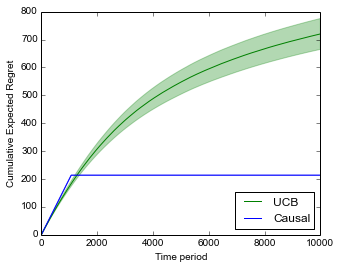
\includegraphics[width=.5\textwidth]{explore_exploit}
\end{figure}

\pagebreak

\section{Generalizing to unbalanced $\boldsymbol{q}$}

\subsection{Option 1: Targeted sampling during exploration phase}

The key fact we were utilizing to draw conclusions about multiple arms during each timestep of the explore phase is that, given our assumed causal structure, $P(Y|do(X_i=j)) = P(Y|X_i=j)$ 

If we do some form of targeted sampling, where we say opt to select each action $I = do(X_a = b)$ some specified number of times $\tau_{ab}$, then we can no longer estimate $P(Y|X_i=j)$ simply by from the proportion of successes given $X_i=j$. 

\eqn {
P(Y|do(X_i=j)) &= P(Y|X_i = j)\\
 &= \sum_{b}P(Y|X_i = j,X_a = b)P(X_a = b|X_i = j) \\
 &= \sum_{b}P(Y|X_i = j,X_a = b)P(X_a = b), \; \forall \, a \in \{1...K\}/i \text{ as } X_a \ci X_i\\
 \label{eqn:marginalizedEstimator}
 &= \sum_{b}P(Y|X_i = j,do(X_a = b))P(X_a = b) 
}

Define $\mu^{ij} = E[Y|X_i=j] = P(Y|X_i=j)$

Let $\hat{\mu}_a^{ij}$ be an estimator for $\mu^{ij}$ based on samples where the intervention was on variable $a$.
\eqn {
\hat{\mu}_a^{ij} &=
\begin{cases}
\label{eqn:marginalizedEstimator2}
\frac{1}{q_i(j)}\left(\frac{m_{a,1}^{ij}}{\tau_{a1}}q_a+\frac{m_{a,0}^{ij}}{\tau_{a0}}(1-q_a)\right) & \text{if } a \neq{i} \\
\frac{m_{i,j}^{ij}}{\tau_{ij}} & \text{if } a=i \\
\end{cases}\\
}

where 

\eqn{
m_{a,b}^{ij} &= \sum_{s \in \{t:I_t=(a,b)\}} Z_{ab,s}^{ij} \text{ and,}\\
Z_{ab,s}^{ij} &= \ind{X_{i,s} = j,Y_s=1} \in \{0,1\}
}

For each arm, specified by the tuple $i,j$, we now have $K$ estimators $[\hat{\mu}_1^{ij}...\hat{\mu}_K^{ij}]$ which we wish to combine to form a single estimator $\hat{\mu}^{ij}$. We will pool them as a weighted average with weights we can optimize based on the $q's$ so as to minimize the variance of the estimator.

\eqn{
\hat{\mu}^{ij} = \sum_{a=1}^K w_{a} \hat{\mu}_{a}^{ij} \;\;\text{, where } \sum_{a=1}^K w_a = 1
}

Putting everything together,

\eqn{
\hat{\mu}^{ij} = \frac{w_i}{\tau_{ij}}\sum_{s \in \{t: I_t = (i,j)\}} Z_{ij,s}^{ij} + \sum_{a \neq i} \left(\frac{w_a}{q_i(j)}\left[ \frac{q_a}{\tau_{a1}}\sum_{s \in \{t:I_t=(a,1)\}} Z_{a1,s}^{ij}+  \frac{1-q_a}{\tau_{a0}}\sum_{s \in \{t:I_t = (a,0)\}} Z_{a0,s}^{ij} \right] \right)
}

We now need to show $E[\hat{\mu}^{ij}] = \mu^{ij}$ and get a high probability bound for their difference. For the latter, lets try and use McDiarmids Inequality. 

McDiarmid's Inequality states:
If $Z_i \ci Z_j$ and 
\eqn{
|\phi(Z_1...Z_i...Z_N) - \phi(Z_1...Z_i^{'}...Z_N)| < c_i \;\; \forall i
}
\eqn{
\label{eqn:McDiarmid}
& P\left(|\phi(\boldsymbol{Z}) - E[\phi(\boldsymbol{Z})]| \geq \epsilon \right) \leq 2 \exp \left(-\frac{2 \epsilon^2}{\sum_{i}c_i^2} \right)\\
& P\left(|\phi(\boldsymbol{Z}) - E[\phi(\boldsymbol{Z})]| \geq 
\sqrt{\frac{\sum_{i}c_i^2}{2}\log{\frac{2}{\delta}}} 
\right) \leq \delta
}

For our problem, $\hat{\mu}^{ij} = \phi(\boldsymbol{Z}^{ij})$. All the $Z's$ are independent as they correspond indicator functions over the results at different timesteps. 

\eqn{
|\phi(...Z_{ij,s}^{ij}...) - \phi(...Z_{ij,s}^{'ij}...)| & \leq \frac{w_i}{\tau{ij}}\;\;\;\; \leftarrow \tau_{ij} \text{ such $Z$'s}\\
|\phi(...Z_{a1,s}^{ij}...) - \phi(...Z_{a1,s}^{'ij}...)| & \leq \frac{w_a q_a}{q_i(j)\tau_{a1}} \;\;\;\; \leftarrow \tau_{a1} \text{ such $Z$'s for each $a$}\\
|\phi(...Z_{a1,s}^{ij}...) - \phi(...Z_{a1,s}^{'ij}...)| & \leq \frac{w_a (1-q_a)}{q_i(j)\tau_{a0}} \;\;\;\; \leftarrow \tau_{a0} \text{ such $Z$'s for each $a$}
}

\eqn{
\label{eqn:sum_ci}
\sum_l c_l^2 = & \frac{w_i^2}{\tau_{ij}} + \sum_{a \neq i}\frac{w_a^2}{q_i(j)^2}\left(\frac{q_a^2}{\tau_{a1}} +\frac{(1-q_a)^2}{\tau_{a0}}  \right)\\
= & \sum_{a=1}^K w_a^2 f(a) \text{, where} \\
f(a) =& \begin{cases}
\frac{1}{q_i(j)^2}\left(\frac{q_a^2}{\tau_{a1}}+  \frac{(1-q_a)^2}{\tau_{a0}}\right)  & a \neq i\\
\frac{1}{\tau_{ij}} & a = i
\end{cases} 
}

We want to select weights to minimize equation \ref{eqn:sum_ci} so as to achieve as tight a bound as possible in equation \ref{eqn:McDiarmid}.

Applying Legrange Multipliers

\eqn {
w_a & = \frac{1}{f(a)\sum_a \frac{1}{f(a)}} \\
\label{eqn:min_sum_ci}
\sum_i c_i^2 & = \frac{1}{\sum_a \frac{1}{f(a)}}
}

Substitution \ref{eqn:min_sum_ci} back into \ref{eqn:McDiarmid}

\eqn {
& P\left(|\hat{\mu}^{ij} - \mu^{ij}| \geq \epsilon \right) \leq 2 \exp \left(-2 \epsilon^2 \sum_{a=1}^K \eta_a^{ij} \right)\\
& \eta_a^{ij} = \begin{cases}
\frac{\tau_{a1} \tau_{a0} q_i(j)^2}{\tau_{a1}(1-q_a)^2+\tau_{a0}q_a^2} & a \neq i\\
\tau_{ij} & a = i
\end{cases} \\
}

Substituting this into \ref{eqn:probDeltaToLarge}

\eqn{
P(\Delta_{\hat{i^*}} > D) \leq 2 \sum_{(i,j)} exp\left({-\frac{D^2}{2} \sum_{a=1}^K \eta_a^{ij}}\right)
}

\eqn{
R_2 \leq (T-h)\left(D+2 \sum_{(i,j)} exp\left({-\frac{D^2}{2} \sum_{a=1}^K \eta_a^{ij}}\right) \right)
}

Looking at the second term

\eqn{
 \sum_{(i,j)} exp\left(-\frac{D^2}{2} \left( \tau_{ij} + q_{ij}^2 \sum_{a \neq i} \frac{\tau_{a1}\tau_{a0}}{\tau_{a1}(1-q_a)^2+\tau_{a0}q_a^2}  \right) \right)
}

Now let $\tau_a = \tau_{a1}+\tau_{a0}$ then $\frac{\tau_{a1}\tau_{a0}}{\tau_{a1}(1-q_a)^2+\tau_{a0}q_a^2}$ is maximized if $\tau_{a1} = q_a \tau_a$

Changing the ratio will only otherwise effect the terms that have where $a = i$. So compare those two terms ...

\eqn{
exp(-\frac{D^2}{2}(\tau_{\alpha 1}+q_\alpha g) + exp(-\frac{D^2}{2}(\tau_{\alpha 0}+(1-q_\alpha)g)
}

minimize this subject to the constraint, hmm seems to give and on the face of it different answer. 

Consider splitting it up so that we sum first over the terms where $j = 1$ then over the terms where $j = 0$ (may be clearer). 


\pagebreak




\subsection{Option 2: Three stage algorithm}
\begin{enumerate}
\item Observe randomly
\item Play low probability arms
\item Pick best and exploit
\end{enumerate}

\pagebreak

\end{document}


